\documentclass[main.tex]{subfiles}
\begin{document}
\chapter{Emulation of hadron-hadron initiated matrix elements}
\label{chapter:fame3}

\section{Motivation}
In the previous two chapters, we detailed the emulation of $e^{+}e^{-}$
annihilation tree-level matrix elements and NLO QCD k-factors. We
have shown that in $e^{+}e^{-}$ annihilation processes we are able to
construct emulators that accurately reproduce the matrix elements,
whilst keeping the evaluation time much lower than existing matrix
element providers.

The Large Electron Positron collider (LEP) was the last high energy
$e^{+}e^{-}$ collider to be in operation with data collection
terminating in 2000 to prepare for the LHC. Lepton-lepton colliders
planned for the future \cite{Faus-Golfe:2022cgm} are not scheduled
to begin operating for at least another decade. Therefore, we turn
our focus to researching techniques to make predictions more efficient
for the LHC, which will be collecting data until the end of the 2030s,
namely, adapting the factorisation-aware model for hadronic collisions.
To showcase the extension to hadronic collisions, we consider several
partonic channels contributing to $Z+4$ and 5 jets production,
and $t\bar{t}+3$ and 4 jets at leading order. These high-multiplicity
processes are of particular importance for physics at the LHC as
they contribute to the background of BSM searches. Furthermore,
these processes typically have very low unweighting efficiencies.

In Ref.~\cite{Danziger:2021eeg} a novel two-stage unweighting
procedure was introduced that used a lightweight neural network
as a surrogate model for the full event weight. This procedure utilises
the rapid evaluations of the surrogate model to first unweight a trial event,
then correct for the mismatch by re-weighting with the full event weight,
where this second re-weighting step has a much higher efficiency.
The authors showed that it was possible to accelerate event unweighting
with this procedure but found that for some processes this procedure
was slower than the standard one-step rejection sampling
(see Section~\ref{sec:unweighting}). In this chapter
we explore whether a more accurate emulation of matrix elements via
the use of the factorisation-aware neural network model would lead
to further acceleration of event unweighting and realise an improvement
for the cases where it did not.

The layout of this chapter is as follows. In Section~\ref{sec:pp_dipoles}
we detail the extension of the model applied in Chapters~\ref{chapter:fame1}
and \ref{chapter:fame2} to hadronic collisions. The novel two-step unweighting
procedure introduced in Ref.~\cite{Danziger:2021eeg} is recapped in
Section~\ref{sec:twostep}. The application of the factorisation-aware
model in this two-step procedure, and implementation in the {\Sherpa} event
generator framework will be discussed in Section~\ref{sec:fame_sherpa}.
In Section~\ref{sec:pp_results} we will showcase the emulator accuracy
and display the acceleration in the generation of unweighted events.
Finally, we will conclude the chapter in Section~\ref{sec:pp_conclusion}
by summarising our findings.

\section{Neural network emulator framework}\label{sec:pp_dipoles}
\subsection{Extension of ansatz to hadronic collisions}\label{sec:pp_ansatz}
The methodology introduced in Chapter~\ref{chapter:fame1}
for emulating $e^{+}e^{-}$ annihilation matrix elements can be straightforwardly
adapted to hadronic collisions by accounting for the radiation
coming from the initial-state partons. This is achieved by extending
the set of dipole functions in the ansatz of the colour
and helicity summed $(n+1)$-body matrix element. The ansatz
is a sum over all permutations of dipole functions relevant
for a given channel, each coming with a corresponding coefficient.
It is given by
\begin{equation}
    |\mathcal{M}_{n+1}|^{2} = \sum_{\{ijk\}} C_{ijk}D_{ij,k} \, ,
    \label{eqn:pp_ansatz}
\end{equation}
where emitter and spectator partons, denoted by $i$ and/or $k$,
can now be initial- and final-state partons.
Therefore, the set of dipoles $D_{ijk}$ now includes the final-final (FF),
final-initial (FI), initial-final (IF), and initial-initial (II) dipoles,
as opposed to just the FF dipoles for $e^{+}e^{-}$ annihilation.
The coefficients $C_{ijk}$, which are more well-behaved than
the matrix element in the soft and collinear limits, are
fitted by the neural network and can be interpreted as reduced matrix
elements. These coefficients are the outputs of the neural network,
which forms an approximation of the matrix element once combined with
the appropriate dipole functions.

An additional extension that we study in this chapter is the
inclusion of massive dipoles in the ansatz of the matrix element.
This enables the examination of pure QCD processes with massive
particles which is of particular importance for top quark pair
production with jets. To that end, we include the massive FF, FI,
and IF dipoles into the ansatz in Eq.~(\ref{eqn:pp_ansatz}).
The massive dipole functions are
generalisations of their massless counterparts, meaning it would
be possible to only use the massive dipole functions for simplicity.
However, only using the massive dipoles when a dipole contains a
massive parton saves on computational costs as the massless dipole
functions are cheaper to evaluate.

To showcase these extensions, we emulate a selection of partonic
channels at tree-level for $Z+4$ and 5 jets, and $t\bar{t}+3$ and 4 jets
production at the LHC. We summarise the partonic channels considered
in Table~\ref{table:pp_partonic_channels}.
Together, these processes allow us to examine the performance
of the extensions detailed above.
We note that with all massless and massive dipoles implemented
into the modelling framework, it is in principle possible to
take advantage of the factorisation-aware model to cover
QCD-enhanced behaviour at tree-level.

\begin{table}
    \centering
    \begin{tabular}{cc}
        \toprule
        Process & Partonic channel(s) \\
        \midrule
        $Z+4j$ & $gg \rightarrow e^{-}e^{+}ggd\bar{d}$ \\
        \midrule
        $Z+5j$ & $gg \rightarrow e^{-}e^{+}gggd\bar{d}$ \\
        \midrule
        $t\bar{t}+3j$ & \makecell{$u\bar{u} \rightarrow t\bar{t}gd\bar{d}$ \\ $gg \rightarrow t\bar{t}ggg$} \\
        \midrule
        $t\bar{t}+4j$ & $ug \rightarrow t\bar{t}gggu$ \\
        \bottomrule
    \end{tabular}
    \caption{List of partonic channels considered in this chapter.}
    \label{table:pp_partonic_channels}
\end{table}

\subsection{Generation of data}\label{sec:pp_data}
Data is generated using the {\Sherpa} event generator
with the {\Amegic} matrix element generator.
Below we list the selection criteria for the phase-space sampling.

\subsubsection*{Z+jets}
For $Z$ boson production in association with jets,
we consider the partonic channels $g g \to e^- e^+ g g d \bar{d}$
and $g g \to e^- e^+ g g g d \bar{d}$ at leading order, representing
tree-level contributions to $Z+4$ jets and $Z+5$ jets production
at the LHC, respectively. The phase-space sampled for generating training
and testing data is constrained by requiring a dilepton invariant
mass $m_{e^- e^+} > \SI{66}{\giga\electronvolt}$ and four or
five anti-$k_t$ jets~\cite{Cacciari:2008gp} with radius parameter
$R = 0.4$ and $p_{T,j} > \SI{20}{\giga\electronvolt}$.
We consider a proton-proton centre-of mass energy of
$\sqrt{s} = \SI{13}{\tera\electronvolt}$ and use the
NNPDF-3.0 NNLO PDF set~\cite{NNPDF:2014otw}.

\subsubsection*{$t\bar{t}$+jets}
For top quark pair production, we consider three partonic channels that contribute to
$t\bar{t}+3$ jets and $t\bar{t}+4$ jets in proton-proton
collisions. These are pure QCD processes with massive particles
which pose a challenge due to the top quarks carrying colour
charge, meaning there is a significant proliferation of Feynman
diagrams when considering their jet-associated production.
For the processes contributing
to $t\bar{t}+3$ jets we require three anti-$k_t$ jets
with $R=0.4$ and $p_{T,j} > \SI{20}{\giga\electronvolt}$.
The phase-space of the process $u g \to t \bar{t} g g g u$
contributing to $t\bar{t}+4$ jets is constrained by requiring
four staggered anti-$k_t$ jets with $R=0.4$, $p_{T,1} > \SI{100}{\giga\electronvolt}$,
$p_{T,2} > \SI{50}{\giga\electronvolt}$, $p_{T,3} > \SI{40}{\giga\electronvolt}$,
and $p_{T,4} > \SI{20}{\giga\electronvolt}$. We do not impose
phase-space cuts for the external top quarks. They are
treated as on-shell in the matrix element calculation,
$p_t^2 = p_{\bar{t}}^2 = m_t^2$ with $m_t = \SI{173.4}{\giga\electronvolt}$,
and only decayed a posteriori.

\subsection{Constructing the emulator}\label{sec:pp_emulator}
The emulator is a dense neural network built using the {\Keras} API
to the {\TensorFlow} backend, and is deployed using the {\ONNX} runtime.
The network consists of four hidden
layers, each containing 128 nodes. We use the swish activation function
for all layers, and initialise node weights according to the Glorot uniform
distribution. We use the data generated from the {\Sherpa} event
generator (described above in Section~\ref{sec:pp_data})
to fit the neural network by minimising the mean squared error.
Training is optimised with the Adam optimiser with an initial
learning rate of $10^{-3}$. Learning rate is reduced by a factor
of 0.7 during training when validation loss shows no improvement
for 30 epochs, and model training is terminated once there is no
improvement in the validation loss after 60 epochs. We summarise
the neural network hyperparameters in Table~\ref{table:pp_hyperparameters}.

\begin{table}
    \caption{Summary of hyperparameters for the neural network
    employed to emulate matrix elements for all partonic channels in
    Table~\ref{table:pp_partonic_channels}.}
    \begin{center}
        \begin{tabular}{ll}
            \toprule
            Parameter & Value \\
            \midrule
            Hidden layers & 4 \\
            Nodes in hidden layers & 128 \\
            Activation function & swish \cite{Hendrycks2016BridgingNA,DBLP:journals/corr/abs-1710-05941}\\
            Weight initialiser & Glorot uniform \cite{pmlr-v9-glorot10a} \\
            Loss function & MSE \\
            Batch size & 512 \\
            Optimiser & Adam \cite{Kingma:2014vow} \\
            Initial learning rate & $10^{-3}$ \\
            Callbacks & {\EarlyStopping}, {\ReduceLROnPlateau} \\
            \bottomrule
        \end{tabular}
    \end{center}
    \label{table:pp_hyperparameters}
\end{table}

As inputs to the neural network, we feed in: the 4-momenta of initial-
and final-state particles, the phase-space mapping variables for each
class of dipole function\footnote{The mapping variables for FF, FI, IF, II dipoles are $y_{ij,k}$ (Eq.~(\ref{eqn:y_ijk})), $x_{ij,a}$ (Eq.~(\ref{eqn:x_ija})), $x_{ik,a}$ (Eq.~(\ref{eqn:x_ika})), and $x_{i,ab}$ (Eq.~(\ref{eqn:II_mapping})), respectively.},
and the kinematic invariants $s_{ij}$ for all pairs of particles in
the process. We refer to all phase-space mapping variables
as $y_{ij,k}$ for brevity, following the notation of
Eq.~(\ref{eqn:pp_ansatz}). To aid the network in training, we preprocess
the phase-space mapping variables in the following manner\footnote{Since we do not
have top quarks in the initial-state, we do not mention massive IF, or II dipoles in Eq.~(\ref{eqn:pp_mapping_transform}).}
\begin{equation}
    y_{ij,k} \rightarrow
    \begin{cases}
        \log(y_{ij,k})   & \text{if massive FI dipole} \, , \\
        \log(1-y_{ij,k}) & \text{if massless FI, IF, or II dipole} \, ,\\
        \log(y_{ij,k})   & \text{otherwise (massless FF dipole)} \, ,
    \end{cases}
    \label{eqn:pp_mapping_transform}
\end{equation}
such that their distributions have similar shape and width. The kinematic invariants
are also transformed with the logarithm as they can span many orders
of magnitude. All inputs are standardised to zero mean and unit variance,
with each component of the 4-momenta being standardised separately.

The target matrix elements are preprocessed by the transformation
\begin{equation}
    |\mathcal{M}_{n+1}|^{2} \rightarrow \mathrm{arcsinh}\left(\dfrac{|\mathcal{M}_{n+1}|^{2}}{S_{\mathrm{pred}}}\right) \, ,
    \label{eqn:pp_me_transform}
\end{equation}
where $S_{\mathrm{pred}}$ is the prediction scale taken to be the
minimum matrix element in the training set. The raw outputs of the
neural network, $c_{ijk}$, are transformed to the coefficients appearing
in the ansatz via the transformation
\begin{equation}
    C_{ijk} = S_{\mathrm{coef}} \times \sinh(c_{ijk})
    \label{eqn:pp_coefs_transform}
\end{equation}
where $S_{\mathrm{coef}}$ is the coefficient scale, defined
as $S_{\mathrm{pred}}/S_{\mathrm{dipole}}$. The dipole scale,
$S_{\mathrm{dipole}}$, is the representative value of a dipole,
which we take to be the median of all dipoles in the training set.
A schematic diagram of the neural network is given in Figure~\ref{fig:pp_nn}.

\begin{figure}
    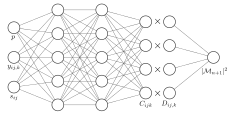
\includegraphics[scale=0.6]{fame3/nn_diagram.pdf}
    \caption{Schematic diagram of neural network architecture
     showing inputs: phase-space points $p$, phase-space mapping
     variables $y_{ij,k}$ and kinematic invariants $s_{ij}$.
     The outputs are the fitted coefficients $C_{ijk}$.}
    \label{fig:pp_nn}
\end{figure}

In Chapters~\ref{chapter:fame1} and \ref{chapter:fame2}, the final
predictions made for the matrix elements were the mean of an
ensemble of independent replica models.
Here we train 10 replica models to monitor the convergence of training,
however, we select only the model with lowest validation loss for
predictions. As a demonstration of model convergence, the training
and validation loss of 10 replica models for the
$gg \rightarrow e^{-}e^{+}ggd\bar{d}$ channel is shown in
Figure~\ref{fig:pp_loss_plot}. This convergent behaviour is
also seen in the other partonic channels.

\begin{figure}
    \includegraphics[width=\linewidth]{fame3/training_loss_curves.pdf}
    \caption{Training and validation loss for the models emulating
    $gg \rightarrow e^{-}e^{+}ggd\bar{d}$ matrix elements. We have
    plotted the mean of the 10 losses as the solid line, with the bands
    indicating the standard error across these 10 models.
    The minimum training and validation loss quoted is for the best
    performing model.}
    \label{fig:pp_loss_plot}
\end{figure}

The rationale behind using an ensemble of models is to dampen the
effects of random model initialisation, to reduce the effects of
stochasticity of the training process, and to provide an estimation
of the uncertainty of the neural network prediction. Additionally, the ensembling
approach has the advantage of providing, in general, a more robust
prediction than a single model, however, that comes at the price
of greater evaluation times. In this chapter where we intend to use the
trained network in an application where speed is a bottleneck, we
have observed that using a single neural network is most performant.
This can be attributed to the fact that there is diminishing returns
in ensembling models, as there is overlapping information from each
replica model. On the other hand, the evaluation time grows linearly
with the number of models in the ensemble, meaning a single
accurate model strikes a good balance between speed and accuracy.
Additionally, the uncertainty associated with the network predictions
is not relevant for the application presented in this chapter as the
network is used in an intermediary step of a larger calculation.

Since we are interested in reducing evaluation time of the neural
network, it is natural to wonder whether it is worth trading
off even more accuracy for speed in the form of reducing the size of the
neural network. A smaller network with fewer nodes/layers would reduce
the size of the weight matrices used during predictions, representing an
increase in throughput.
However, the neural network is deployed using the highly optimised
{\ONNX} runtime where we have observed that more compact networks
do not reduce evaluation time by very much at all, whereas there
is an appreciable decrease in accuracy, leading to lower efficiency
of the second unweighting step described below.

\section{Novel two-stage unweighting algorithm}\label{sec:twostep}
Generation of unweighted events is carried out via rejection sampling,
as outlined in Section~\ref{sec:unweighting}, where event weights
are normalised by the maximal event weight, $w_{\mathrm{max}}$,
before being compared to a uniform random number $r \in [0,1]$. If
$w / w_{\mathrm{max}} < r$ then events are accepted and assigned
a unit-weight. This procedure means that small event weights
have a lower probability of being accepted, whereas larger event weights
are more likely to be accepted. An issue with unweighting is that
the number of accepted events, $N$, is generally much lower than the
number of trial events, $N^{\mathrm{trials}}$. This is encapsulated in
the unweighting efficiency
\begin{equation}
    \epsilon = \dfrac{N}{N^{\mathrm{trials}}} \approx \dfrac{\langle w \rangle_{N^{\mathrm{trials}}}}{w_{\mathrm{max}}} \; \text{for large} \; N^{\mathrm{trials}} \, ,
    \label{eqn:pp_unweighting_efficiency}
\end{equation}
where $\langle w \rangle_{N^{\mathrm{trials}}}$ is the mean event weight
over all trials. The inverse $1 / \epsilon$ gives the average number of
trial events required to accept one unit-weight event. The rejection
sampling algorithm depends
on the maximal event weight, $w_{\mathrm{max}}$, which cannot usually be
exactly determined given finite statistics. Furthermore, it is possible to
have large outlier event weights which when taken to be $w_{\mathrm{max}}$ would
lead to excessively low unweighting efficiencies.

One method to avoid this issue is to define a reduced $w_{\mathrm{max}}$
and accept overweights, meaning weights with $w > w_{\mathrm{max}}$
are accepted but are assigned with a correction factor
$\tilde{w} = w / w_{\mathrm{max}}$.
This process leads to partially
unweighted events and is summarised in Algorithm~\ref{alg:partial_unweighting}.
It is the default method to generate unweighted events in the {\Sherpa}
framework.
A systematic approach to reducing $w_{\mathrm{max}}$
is the per-mille quantile reduction method which defines $w_{\mathrm{max}}^{\mathrm{p.m.}}$
such that overweights contribute at most 0.1\% to the total cross-section.

\begin{algorithm}
    \caption{Rejection sampling for generating partially unweighted events.}
    \label{alg:partial_unweighting}
    \While{unweighting}{
        generate random phase-space point $\mathbf{x}$\;
        evaluate event weight $w \gets w(\mathbf{x})$\;
        generate uniform random number $r \gets$ Random(0, 1)\;
        \If{$w / w_{\mathrm{max}} > r$}{
            \KwRet $\mathbf{x}$ and $\tilde{w} \gets \max(1,\; w / w_{\mathrm{max}})$\;
        }
    }
\end{algorithm}

Whilst the partial unweighting approach increases overall unweighting efficiency,
it remains low for high-multiplicity processes.
A novel two-step unweighting procedure was introduced in Ref.~\cite{Danziger:2021eeg}
to accelerate unweighted event generation. This procedure is formed of two separate
unweighting steps. The first unweighting step uses
a lightweight surrogate neural network model, which approximates the event weight,
to rapidly unweight the trial event. Given that the surrogate model is in general imperfect, the
second unweighting step corrects for this by calculating the exact event weight
and applying a correction factor, meaning the final event accepted is exact and has
unit-weight. This second step is similar to the process of dealing with overweights described
above.
The advantage of this approach is that the expensive exact event weight is only
evaluated once the first step accepts a trial event. This means that the number of 
expensive exact event weight computations is drastically reduced for a sufficiently accurate
surrogate model, hence accelerating unweighted event generation. In Ref.~\cite{Danziger:2021eeg},
the authors used a surrogate model to approximate the full event weight, 
$w = J_{\mathrm{PS}} |\mathcal{M}|^{2}$. In this chapter we explore the possibility
to emulate only the matrix element using the factorisation-aware model detailed in the
previous section, whilst keeping the phase-space weight computation exact.

The two-stage algorithm is outlined in Algorithm~\ref{alg:twostep}, where we have
denoted the matrix element approximation as $|M|^{2}$ in line number 3. This
two-step approach introduces an additional weight, $x_{\mathrm{max}}$, analogous
to the maximal event weight $w_{\mathrm{max}}$. It is the maximum truth-to-prediction
ratio. This could in principle be a large value, so the quantile reduction method
is used to define a more practical $x_{\mathrm{max}}^{\mathrm{p.m.}}$ for more efficient
unweighting in the second step. This will be described in more detail in Section~\ref{sec:fame_sherpa}.
\begin{algorithm}[ht]
    \caption{Two-stage rejection sampling algorithm employing
    a surrogate model to approximate exact event weight.}
    \label{alg:twostep}
    \While{unweighting}{
      generate phase-space point $\mathbf{x}$\;
      calculate approximate event weight $s \gets J_{\mathrm{PS}}|M|^{2}$\;
      generate uniform random number $r_1 \gets$ Random(0, 1)\;
        \tcp{first unweighting step}
        \If{$s / w_{\mathrm{max}} > r_1$}{
          calculate exact event weight $w \gets w(\mathbf{x})$\;
          determine ratio $x \gets w/s$\;
          generate uniform random number $r_2 \gets$ Random(0, 1)\;
            \tcp{second unweighting step}
            \If{$x / x_{\mathrm{max}} > r_2$}{
            \KwRet $\mathbf{x}$ and $\widetilde{w} \gets \max(1, s/w_\text{max})\cdot\max(1, x/x_\text{max})$
            }
        }
    }
\end{algorithm}

The acceleration of this approach can be quantified by the
effective gain factor which is given by
\begin{align}\label{eq:gain_factor}
	f_{\text{eff}} & = \dfrac{T_{\text{standard}}}{T_{\text{surrogate}}} \nonumber \, ,\\
	&= \dfrac{N_{\text{full}}^{\text{trials}} \times \langle t_{\text{full}}
	\rangle}{N_{\text{1st}}^{\text{trials}} \times \left[\langle
			t_{\text{surr}} \rangle + \langle t_{\text{PS}}
		\rangle\right] + N_{\text{2nd}}^{\text{trials}} \times \langle
	t_{\text{ME}} \rangle} \, , \\
	&= \dfrac{1}{\frac{\langle t_{\text{surr}} \rangle + \langle
			t_{\text{PS}} \rangle}{\langle t_{\text{full}} \rangle}
			\times
			\frac{\epsilon_{\text{full}}}{\epsilon_{\text{1st}}
			\epsilon_{\text{2nd}}} + \frac{\langle
		t_{\text{ME}} \rangle}{\langle t_{\text{full}} \rangle} \times
	\frac{\epsilon_{\text{full}}}{\epsilon_{\text{2nd}}}} \nonumber \, .
\end{align}
This effective gain factor can be understood as the ratio of the
average times of the standard unweighting approach, compared to the two-stage
unweighting approach, such that a higher $f_{\mathrm{eff}}$ is desirable.
The time spent in the standard approach is simply the number of trial events,
$N_{\mathrm{full}}^{\mathrm{trials}}$, multiplied by the average evaluation
time of the exact event weight in this sample of trials, $\langle t_{\mathrm{full}} \rangle$.
The total time of the two-stage approach can be split up into two steps.
The first step involves the evaluation of the surrogate model
(including all input computations, pre- and post-processing) and the exact phase-space
weight, $\langle t_{\mathrm{surr}} \rangle$ and $\langle t_{\mathrm{PS}} \rangle$,
for the number of trial events $N_{\mathrm{1st}}^{\mathrm{trials}}$. The second
step involves the evaluation of the exact matrix element (using the phase-space weight
from the previous step to recover the exact event weight), $\langle t_{\mathrm{ME}} \rangle$,
for $N_{\mathrm{2nd}}^{\mathrm{trials}}$ second step trial events.
From the second to the final line of Eq.~(\ref{eq:gain_factor}), we divided the numerator and denominator by
$N_{\mathrm{full}}^{\mathrm{trials}} \times \langle t_{\mathrm{full}} \rangle$
and defined
\begin{align}
    \label{eq:unweighting_efficiencies}
    \epsilon_\text{full} &= \dfrac{N}{N^\text{trials}_\text{full}} \approx \dfrac{\langle w \rangle}{w_{\mathrm{max}}^{\mathrm{p.m.}}} \, , \nonumber \\
    \epsilon_\text{1st} &= \dfrac{N^\text{trials}_\text{2nd}}{N^\text{trials}_\text{1st}} \approx \dfrac{\langle s \rangle}{w_{\mathrm{max}}^{\mathrm{p.m.}}} \, , \\
    \quad \epsilon_\text{2nd} &= \dfrac{N}{N^\text{trials}_\text{2nd}} \approx \dfrac{\langle x \rangle}{x_{\mathrm{max}}^{\mathrm{p.m.}}} \, , \nonumber
\end{align}
where $\langle w \rangle$ is the mean of the weights generated during {\Sherpa}'s
integration run (see Section~\ref{sec:fame_sherpa}),
$\langle s \rangle$ is the mean of the surrogate model predictions
on the test set, and $\langle x \rangle$ is the mean of the corresponding truth-to-prediction ratios.
These efficiencies represent the unweighting efficiencies of the standard
approach, and of the two steps in the two-step approach, respectively.
From the expression of the effective gain factor, Eq.~(\ref{eq:gain_factor}),
we would expect large gains for processes where $\epsilon_{\mathrm{full}}$ is low.
Indeed, this is the case for the high-multiplicity processes we consider. Furthermore,
for a fast and accurate surrogate model, where
$\langle t_{\mathrm{surr}} \rangle \ll \langle t_{\mathrm{full}} \rangle$,
$\epsilon_{\mathrm{1st}} \approx \epsilon_{\mathrm{full}}$, and
$\epsilon_{\mathrm{2nd}} \approx 1$, we would also expect large gains.

\subsection{Implementation in {\Sherpa}}\label{sec:fame_sherpa}
To implement the neural network emulator described in Section~\ref{sec:pp_emulator}
as a surrogate model for the matrix elements in the two-step algorithm
outlined in Section~\ref{sec:twostep},
we need to generate data for training and testing the neural network,
and to use the model to approximate the event weight during the unweighting
process.
Cross-section predictions in {\Sherpa} are made in two phases.
Firstly, there is an optimisation phase which allows the integrator to adapt
to the partonic channel of interest \cite{Kleiss:1994qy}. This is followed by an integration
phase in which the integrator is used to determine the total cross-section.
During this integration phase, weighted events are generated and $w_{\mathrm{max}}^{\mathrm{p.m.}}$
is determined with the quantile reduction method which we describe below.
In the standard partial unweighting procedure, the reduced maximal event weight,
$w_{\mathrm{max}}^{\mathrm{p.m.}}$, is determined by first sorting weights
generated during the integration phase, $\{w_{i}\}$, such that $w_{i} < w_{i+1}$, then requiring
\begin{equation}
    w_{\mathrm{max}}^{\mathrm{p.m.}} = \min\left(w_{j} \; \Bigg| \; \sum_{i=j+1}^{N} w_{i} < 0.001 \sum_{i=1}^{N} w_{i} \right) \, ,
    \label{eq:w_max}
\end{equation}
i.e. find the first weight from $\{w_{i}\}$ such that the sum of all larger weights
contributes at most 0.1\% to the total cross-section.

During the integration phase, 1.5 million events are taken for training
and testing data by saving the 4-momenta, phase-space weights, and matrix
elements. In this chapter we study the emulation of colour and helicity
summed matrix elements, which are evaluated using the {\Amegic} matrix
element provider in {\Sherpa}. From these 1.5 million events, we take 800k events for
training, 200k events for validation during training, and use the final 500k events
for independent testing of the model once it has been trained. The testing
dataset is used to determine the value of $x_{\mathrm{max}}$.
The same quantile reduction method described above can be used to define
a reduced $x_{\mathrm{max}}$, $x_{\mathrm{max}}^{\mathrm{p.m}}$, that allows
for more efficient unweighting in the second step of the two-step procedure
at the expense of overweights.
By sorting the sequence of truth-to-prediction ratios, $\{x_{i}\}$, such that
$x_{i} < x_{i+1}$ and using the same sorting order for $\{s_{i}\}$,
$x_{\mathrm{max}}^{\mathrm{p.m.}}$ is defined as
\begin{equation}
    x_{\mathrm{max}}^{\mathrm{p.m.}} = \min\left(x_{j} \; \Bigg| \; \sum_{i=j+1}^{N} x_{i}s_{i} < 0.001 \sum_{i=1}^{N} x_{i}s_{i} \right) \, .
    \label{eq:x_max}
\end{equation}

This process is repeated for each partonic channel that we study, where each channel
has its own neural network surrogate model.
The {\ONNX} runtime has a simple \texttt{C++} API, meaning it is straightforward to
incorporate the model into a \texttt{C++} workflow. The interface to the {\Sherpa} framework
is then a case of writing wrapper code that takes the phase-space point generated from
{\Sherpa} to compute the model input variables $y_{ijk}$ and $s_{ij}$, make the model
predictions, $C_{ijk}$, and then combines them with the appropriate dipole
functions to form an approximation of the matrix element. This setup can then be
used to perform the two-stage unweighting procedure in Algorithm~\ref{alg:twostep} by calling the
surrogate model for every $|M|^{2}$ evaluation.

\section{Results}\label{sec:pp_results}
In this section, we evaluate the performance of the neural network model by
examining the error distributions for the predictions made with the model.
Following this, we display results for the application in the two-stage
unweighting procedure by quoting effective gain factors, $f_{\mathrm{eff}}$.
\subsection{Emulator error distributions}
In Figure~\ref{fig:pp_err_dists}, we show error distributions for the neural network predictions,
by plotting the prediction-to-truth ratio, $w/s$, for the 500k events in the independent testing
dataset for each channel, as indicated by the legend labels. In the left-hand subplots, we
plot $w/s$ on a linear scale to assess the model performance
in terms of accuracy, whereas on the right-hand subplots we plot $\log_{10}(w/s)$. This allows us to
examine the tails of the distribution which are important for the second unweighting step,
as a large right-handed tail skews the value of $x_{\mathrm{max}}^{\mathrm{p.m.}}$.
All error distributions are centred around the ideal values of 1 or 0, for the left- and
right-hand subplots, respectively, with the distributions having a Gaussian-like distribution
that is narrow.

We see that performance on the channels associated with $Z$+jets production are
generally worse than for the top quark pair production channels. This can be attributed
to the multiplicity of the channels, as increasing multiplicity generally leads to a drop
in accuracy as already discussed in Chapters~\ref{chapter:fame1} and \ref{chapter:fame2}.
At the same multiplicity, the $gg \rightarrow t\bar{t}ggg$ channel presents a more difficult channel
to model than $u\bar{u} \rightarrow t\bar{t}gd\bar{d}$ due to the presence of more
infrared singularities, however, the associated accuracy with this gluon initiated channel
remains higher than for the $t\bar{t}+4j$ case, in line with the assessment above.

To inspect the tails on the right-hand subplots further, we plot 2d histograms of $w/s$
against the value of the event weights. This allows
us to see whether the tails emerge from large weight events, or from small weight events.
This is illustrated in Figure~\ref{fig:pp_2d_hist_z5j} for the $Z+5j$ process as this
is the channel with the lowest accuracy, meaning the other channels are better behaved.
We see that the model is generally well-behaved
for large event weights as the high population bins depicted in yellow, are centred around
the ideal value of 0, and the error distribution is generally contained inside a band.
From this plot, we also see that outlier events depicted in purple are predominately
smaller event weights.

\begin{figure}
    \includegraphics[width=\linewidth]{fame3/ratio_plots.pdf}
    \caption{Error distributions for all partonic channels. All histograms
    are produced from 500k test events. Left: linear
    truth-to-prediction ratio distributions, right: $\log_{10}$ truth-to-prediction
    ratio distributions. The upper two subplots illustrate
    the $Z+4j$ and $Z+5j$ processes, with the lower two subplots illustrating
    the $t\bar{t}+3j$ and $t\bar{t}+4j$ processes.}
    \label{fig:pp_err_dists}
\end{figure}

\begin{figure}
    \includegraphics[scale=0.65]{fame3/z5j_hexbin_w.pdf}
    \caption{Left: 2d histogram of $\log_{10}(w/s)$ against the respective
    event weight, $w$ for the $gg \rightarrow e^{-}e^{+}gggd\bar{d}$ channel.
    Yellow bins represent high population bins, and purple bins represent
    single points. Right: marginal distribution of $gg \rightarrow e^{-}e^{+}gggd\bar{d}$
    event weights.}
    \label{fig:pp_2d_hist_z5j}
\end{figure}

\subsection{Unweighting gains}
With the model performance validated, we move on to discussing
the acceleration of unweighted event generation by using
the neural network emulator as the surrogate model in the two-stage
unweighting procedure.

The amount of acceleration is quantified by the effective gain factor,
$f_{\mathrm{eff}}$, which measures the average time saved to
unweight a sample of events compared to the standard
one-step rejection sampling approach. To determine $f_{\mathrm{eff}}$,
we run through the procedure described in Algorithm~\ref{alg:twostep}
for a number of events in the testing datasets and record
$\langle t_{\mathrm{surr}} \rangle$, $\langle t_{\mathrm{PS}} \rangle$, and
$\langle t_{\mathrm{ME}} \rangle$.
We note that $\langle t_{\mathrm{full}} \rangle = \langle t_{\mathrm{PS}} \rangle + \langle t_{\mathrm{ME}} \rangle$.
Depending on the complexity
of the process, between 10 and 10000 events are unweighted to get a reliable
estimate of these times. Eqs.~(\ref{eq:gain_factor}) and
(\ref{eq:unweighting_efficiencies}) are then used to calculate $f_{\mathrm{eff}}$.

In Table~\ref{table:gain_factors} we quote the timings, efficiencies,
and the computed effective gain factors for all channels,
where we can see the speed up ranges from 14 to up to 366 times
compared to the standard approach. This is due to the rapid
neural network evaluation times and good predictive accuracy leading
to relatively high $\epsilon_{\mathrm{1st}}$ and $\epsilon_{\mathrm{2nd}}$.
Interestingly, the largest
gains are seen for the most computationally expensive processes,
namely, the $Z+5j$ and $t\bar{t}+4j$ processes. This demonstrates
that the surrogate model has managed to accurately model the matrix
elements, and to produce the approximations rapidly. We can
see that $\langle t_{\mathrm{surr}} \rangle$ only scales weakly
with the multiplicity, whereas $\langle t_{\mathrm{ME}} \rangle$
increases very rapidly for more complex final-states.

\begin{table}
    \sisetup{table-auto-round}
    \centering
    \small
    \begin{tabular}{@{}
        l
        S[table-format=1.1e1,scientific-notation]
        S[table-format=1.1e1,scientific-notation]
        S[table-format=1.1e1,scientific-notation]
        S[table-format=1.1e1,scientific-notation]
        S[table-format=1.1e1,scientific-notation]
        S[table-format=1.2]
        l
        @{}}
        \toprule
        \multirow{2}[3]{*}{Process} & \multicolumn{3}{c}{Timings / \unit{\second}} & \multicolumn{3}{c}{Efficiencies} & \multirow{2}
        [2]{*}{$f_{\mathrm{eff}}$} \\
        \cmidrule(lr){2-4} \cmidrule(lr){5-7}
            & $\langle t_{\mathrm{ME}} \rangle$ & $\langle t_{\mathrm{PS}} \rangle$ & $\langle t_{\mathrm{surr}} \rangle$ & $\epsilon_{\mathrm{full}}$ & $\epsilon_{\mathrm{1st}}$ & $\epsilon_{\mathrm{2nd}}$ & \\
        \midrule
        $gg \rightarrow e^{-}e^{+}ggd\bar{d}$ & 0.05394600000000000 & 0.00039500000000000 & 0.00013900000000000 & 0.0155569 & 0.0140033 & 0.374251 & 14 \\
        $gg \rightarrow e^{-}e^{+}gggd\bar{d}$ & 16.21580000000000155 & 0.00570000000000000 & 0.00020000000000000 & 0.0007556797419000464 & 0.0008515348336151582 & 0.2904892762892554 & 269 \\
        \midrule
        $u\bar{u} \rightarrow t\bar{t}gd\bar{d}$ & 0.00525400000000000 & 0.00003500000000000 & 0.00013800000000000 & 0.000872182 & 0.00247838 & 0.2849 & 23 \\
        $gg \rightarrow t\bar{t}ggg$ & 3.26229999999999976 & 0.00090000000000000 & 0.00018300000000000 & 0.00884173 & 0.01514 & 0.5 & 55 \\
        $ug \rightarrow t\bar{t}gggu$ & 51.20000000000000284 & 0.00400000000000000 & 0.00023900000000000 & 0.0014836499653593951 & 0.0015978362349985088 & 0.5704770330576479 & 366 \\
        \bottomrule
    \end{tabular}
    \caption{Unweighting performance measures for all partonic channels.}
    \label{table:gain_factors}
\end{table}

\section{Conclusion}\label{sec:pp_conclusion}
In this chapter we have studied the extension of the factorisation-aware
model from electron-positron annihilation matrix elements explored in
Chapters~\ref{chapter:fame1} and \ref{chapter:fame2} to hadronic collisions.
The model was readily adapted by changing the ingredients in the ansatz
of the matrix element to include the full set of massless dipoles
to account for radiation from the initial-state partons.
Additionally, we included the full set of massive dipole functions to
enable the accurate modelling of matrix elements with massive partons,
in this case top quark pair production.
We have demonstrated that with these additional dipole functions, it is
possible to accurately approximate the matrix elements of high-multiplicity
hadronic processes with well-behaved predictions for large event weights.

We have also showcased an application of the neural network model in
the form of accelerating event unweighting in the {\Sherpa} framework
by using the neural network model in a novel two-stage unweighting procedure.
The performance of this unweighting procedure relied on the fast and accurate
predictions of the model.
We showed that for all partonic channels considered, the unweighting procedure
was accelerated, with the largest gains coming from the most
computationally expensive channels where the effective gain factors
were well over two orders of magnitude.
\end{document}